
The aim of this section is to evaluate the RL framework for mapping a workload to a an SE under training and fine-tuning scenarios. 
We also analyze the effects of the different components of the RL model, such as: GGA module, output masking and node iteration ordering.

The implemented RL approach was able to successfully map the SDF graphs for different programs such as vector add, distance calculation function and Fast Fourier Transform (FFT). 
FFT is widely used by several applications such as digital signal and image processing, pattern recognition, solving partial differential equations, error-correcting codes, and many others \cite{814659}.
FFT has time complexity of $\mathcal{O}(N\log{N})$ and two nested loops.
The outer loop and inner loop have time complexity of $\mathcal{O}(\log{N})$ and $\mathcal{O}(N)$ respectively.
The inner loop is targeted for acceleration.
The inner loop code is optimized and broken down into four SDFs which are shown in \figurename~\ref{fig:ifft_graph}.
The SE device configuration for the following experiments used 16 tiles and a maximum II of six.
Other SE device configurations are possible.

\begin{figure}[tb]
  \centering
  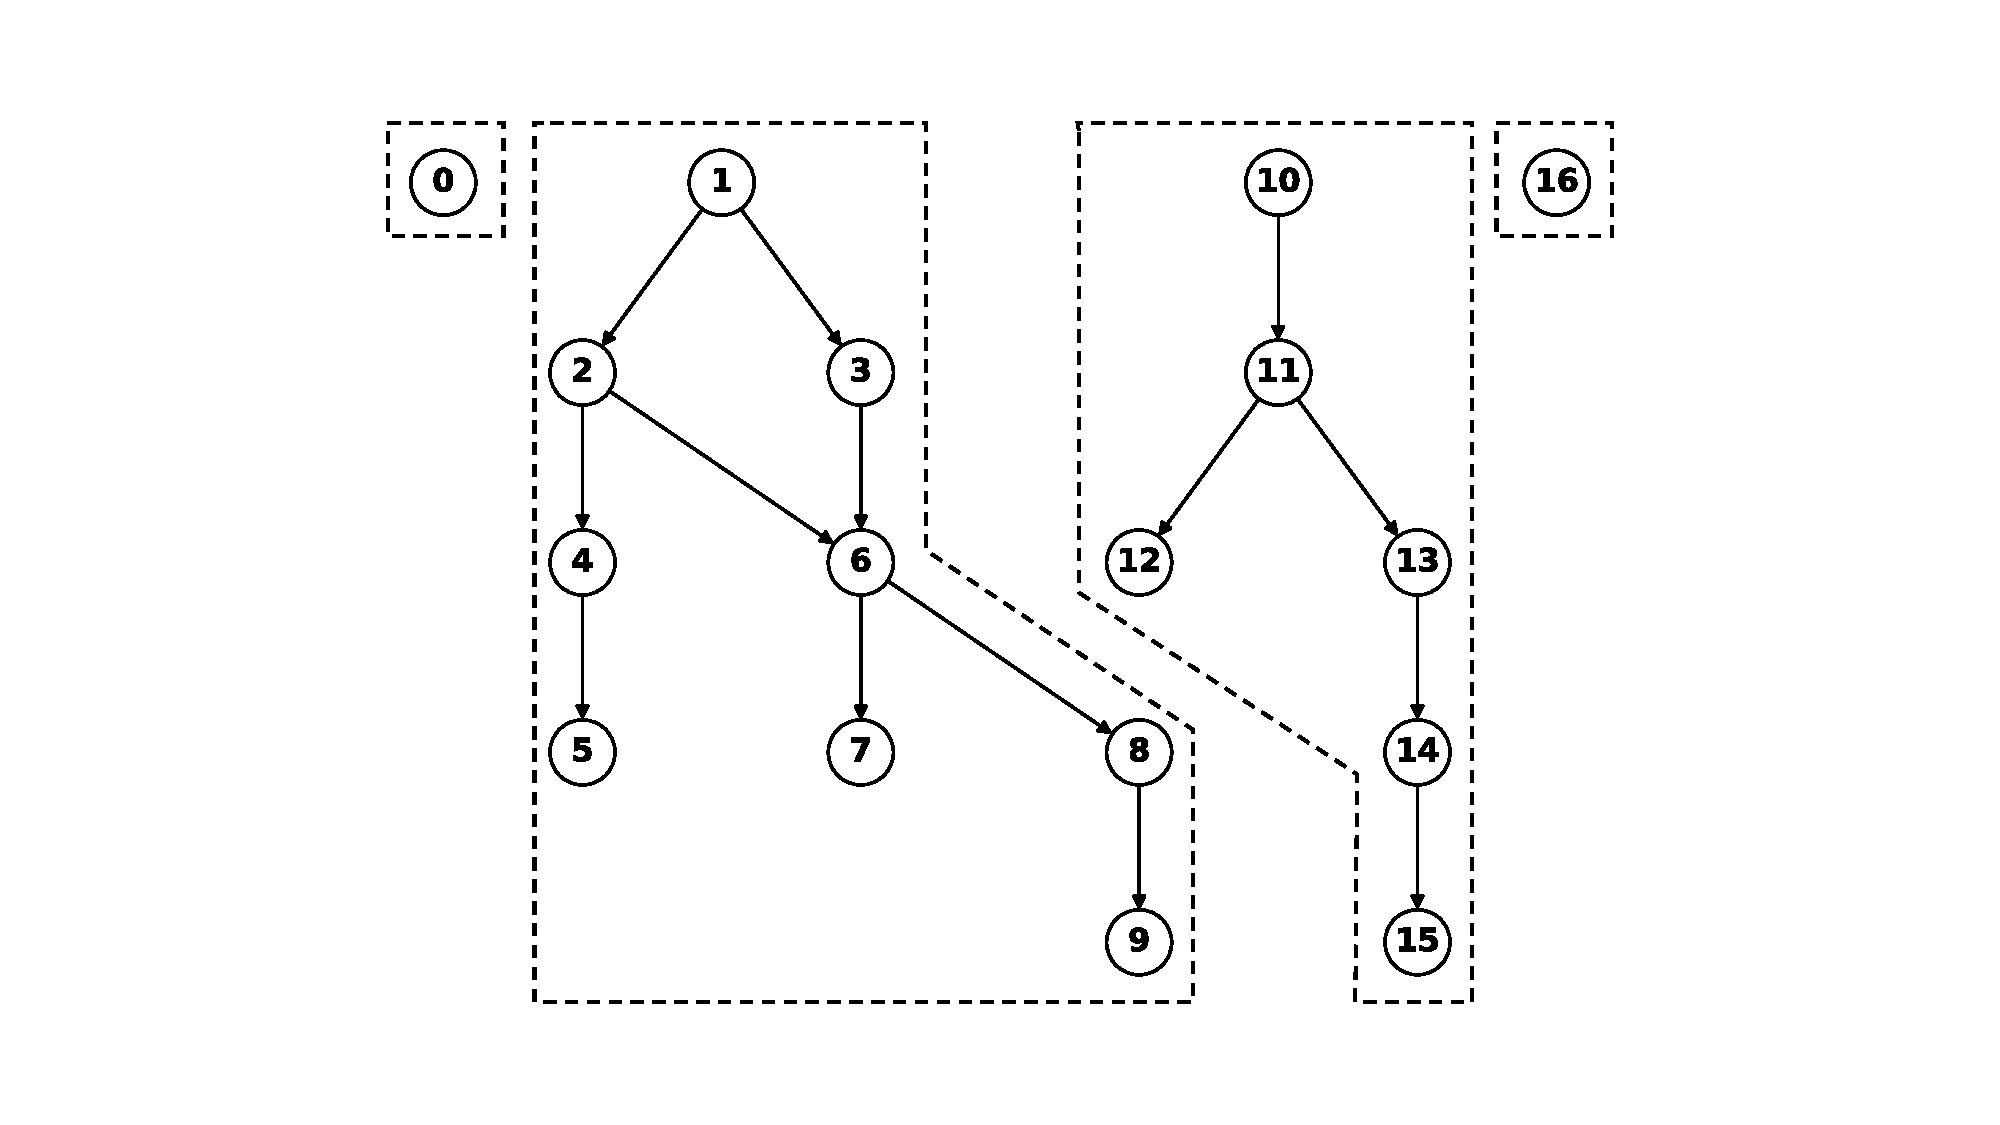
\includegraphics[width=\linewidth]{fig/ifft_graph.pdf}
  \caption{SDF graph of the FFT application.}
  \label{fig:ifft_graph}
\end{figure}

\begin{figure}[tb]
  \centering
  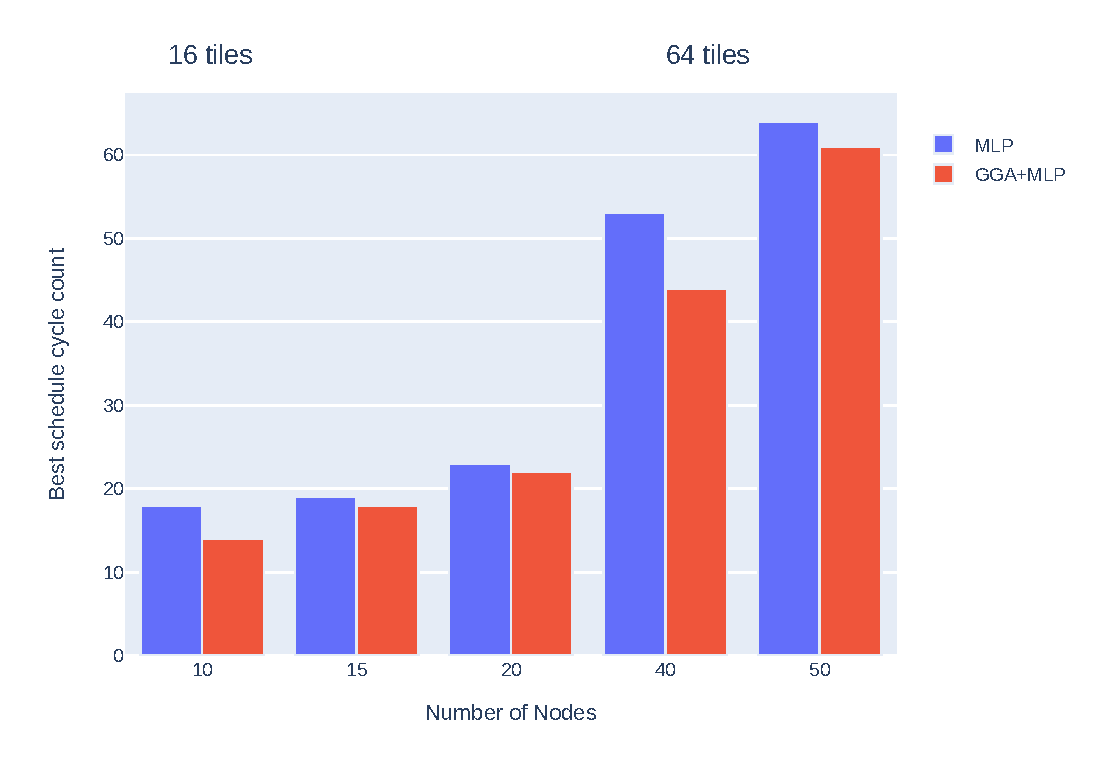
\includegraphics[width=\linewidth]{fig/nodes_graph.pdf}
  \caption{Cycle count for running all nodes in the best mapping given by RL model over 50,000 epochs. 
  PPO baseline MLP model and GGA model were evaluated with computation graphs with increasing number of nodes. 
  A larger device configuration with 64 tiles was used for experiments with SDF graphs with 40 and 50 nodes. }
  \label{fig:nodes_graph}
\end{figure}

\begin{figure}[tb]
  \centering
  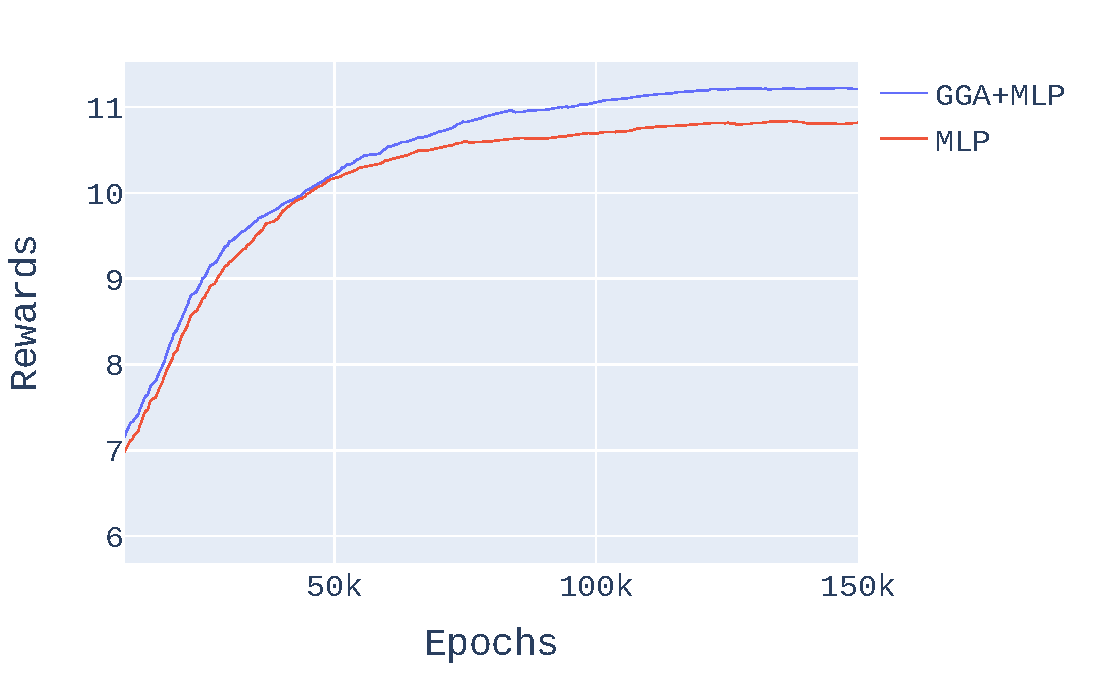
\includegraphics[width=\linewidth]{fig/plot_gnn_atten_ppo.pdf}
  \caption{Effect of using Global Graph Attention (GGA) module for mapping the FFT application on device with 16 tiles. 
  GGA module provides better sample efficiency and higher reward after training. }
  \label{fig:ifft_rewards}
\end{figure}

\begin{figure}[tb]
  \centering
  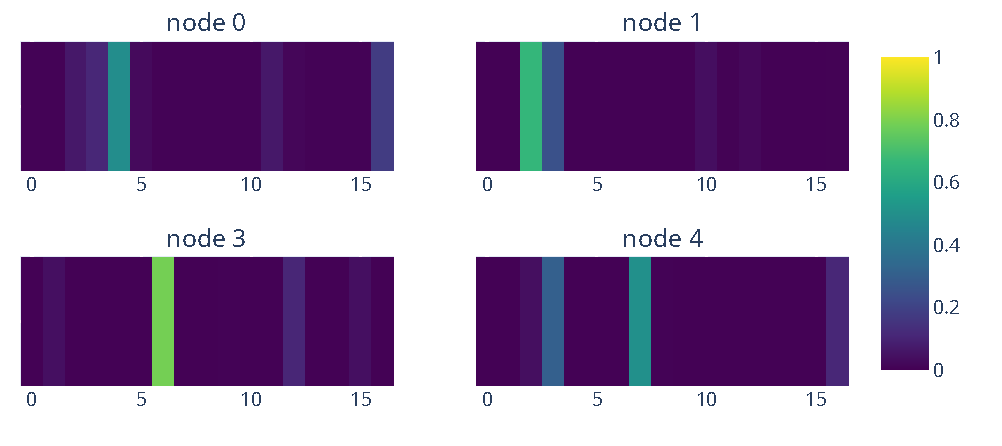
\includegraphics[width=\linewidth]{fig/ifft_attention.pdf}
  \caption{Attention scores from transformer module when placing certain nodes for the FFT application. }
  \label{fig:ifft_attention}
\end{figure}

\begin{figure}[tb]
  \centering
  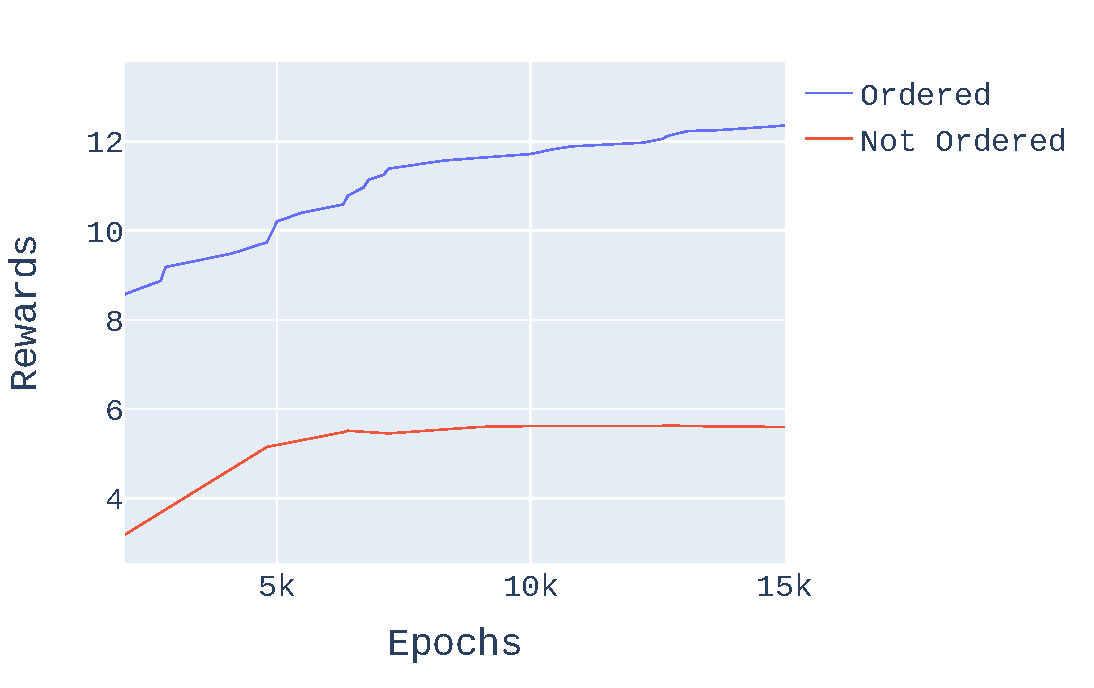
\includegraphics[width=\linewidth]{fig/plot_ordered.pdf}
  \caption{Iterating nodes in topological ordering results in higher reward and eases the placement task. 
 The blue line is the reward curve for when nodes were randomly selected for placement. 
 The red line is the reward curve for when nodes were iterated upon in topological order. 
 The task involved is of placing 15 nodes of an SDF graph onto a device with 16 tiles.}
  \label{fig:ordered_placement}
\end{figure}

\begin{figure}[tb]
  \centering
  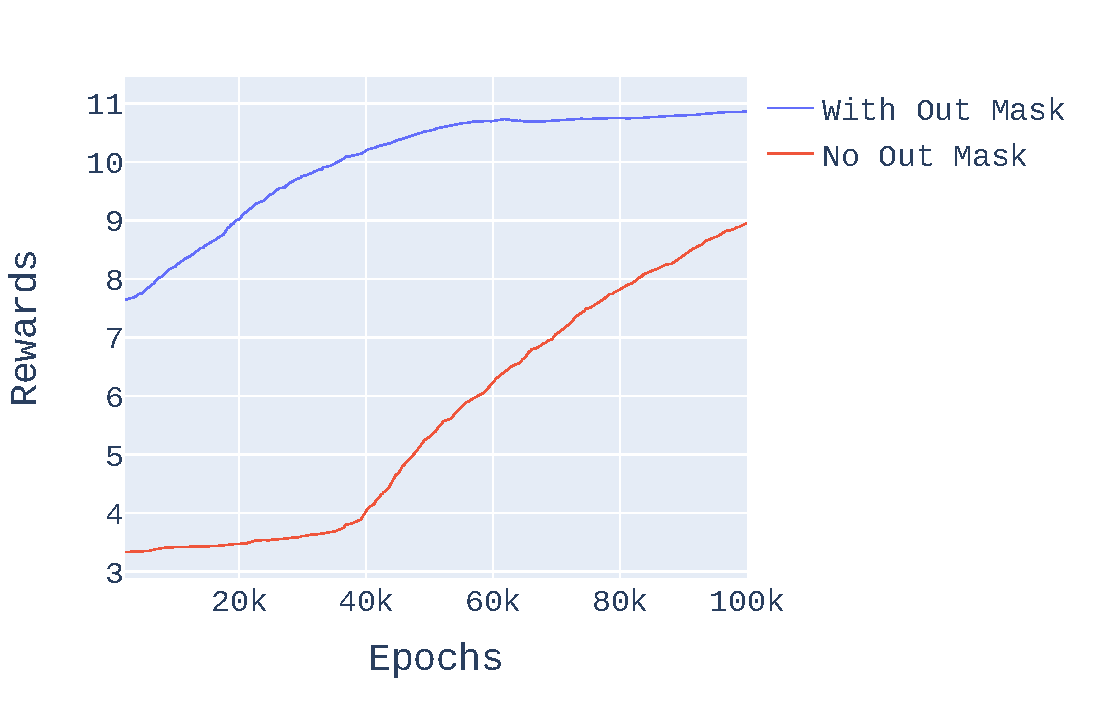
\includegraphics[width=\linewidth]{fig/ifft_masked_nomask.pdf}
  \caption{Reward comparison between node placement with output masking (blue) and without output masking (red).}
  \label{fig:mask_nomask}
\end{figure}

\begin{figure}[tb]
  \centering
  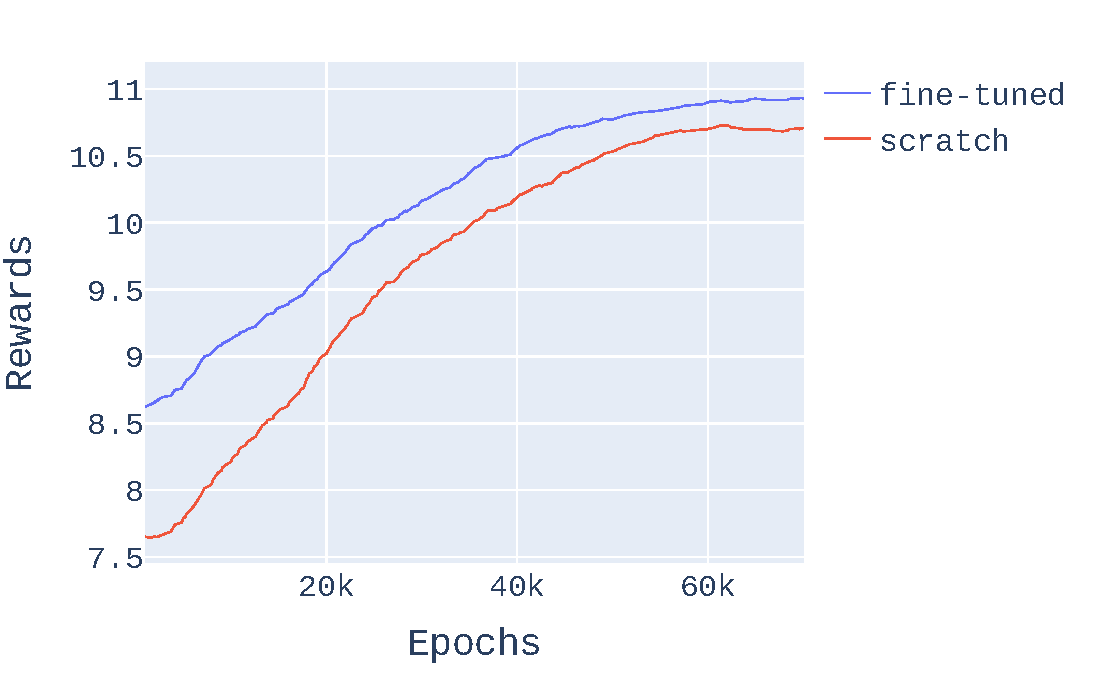
\includegraphics[width=\linewidth]{fig/pretrain_ifft.pdf}
  \caption{Comparison between training RL model from scratch (red) versus fine-tuning a model pre-trained on random graphs (blue). }
  \label{fig:pretrain_ifft}
\end{figure}

We also benchmarked our RL framework against a collection of random directed graphs meant to simulate real life workloads. 
We compare a baseline PPO method composed of three stacked MLPs against an actor model with the proposed GGA module.
We evaluate these models on varying SDF graphs with different complexities by increasing number of nodes in the graph. 
We also tested on a larger device with 64 tiles.
In \figurename~\ref{fig:nodes_graph}, we observe that the RL approach finds mappings for a variety of computation graphs, and GGA improves the best schedule found for the same number of training epochs. 
The GGA also finds an improved schedule in terms of clock cycles taken for a larger device configuration. 
For the results in \figurename~\ref{fig:nodes_graph}, the epochs were limited to 50,000 for both models. 
The cycle count is the number of SE execution steps taken to process all nodes for a mapping, which is calculated from the simulated SE environment. 

\subsection{GGA} \label{sec:GGA_result}

In \figurename~\ref{fig:ifft_rewards}, we see the addition of GGA module provides improved reward and sample efficiency for the FFT application by 10\%. 
The node and states changes for each iteration over all nodes in the SDF graph. The GGA module provides a representation of the entire graph while placing each node.

The attention module assists in highlighting the node dependencies when the RL model is predicting the placement of a node. 
In \figurename~\ref{fig:ifft_attention}, we plot the attention matrix produced by the GGA module when mapping nodes from the FFT application shown in \figurename~\ref{fig:ifft_graph}. 
The x-axis is the node index, the title indices which node is being placed and the color axis indicates attention scale.
For node 1, the model tries to focus on nodes 2 and 3. When placing node 3, the attention slightly shifts to node 6. 
These attention examples matches with expectation that these nodes are related since they have direct data dependencies. 

\subsection{Node Iteration Order}

The iteration order is the sequence in which nodes are fed to the actor model in the RL framework and plays an important role in deciding whether the nodes can be successfully placed or not. 
In \figurename~\ref{fig:ordered_placement}, we observe that iterating over nodes in topological ordering results in higher reward and eases the node placement task. 
On the other hand, when placing the nodes randomly, sometimes nodes get placed before their predecessors are placed and the model needs to predict which tiles the predecessor nodes will be placed on, making training and the learning problem harder.

\subsection{Output Masking}
\label{subsec:output_masking}
Output masking to filter invalid placements has been shown to be effective for RL in game environments \cite{Shengyi_mask}. 
The SE instruction scheduling task has several invalid actions for a given state that add noise to the samples and decision of the RL model, making convergence harder. 
After placement of each node, the succeeding nodes have fewer placement options due to their data dependency with other nodes and device constraints.
Masking invalid placements reduces the search space as each node is being placed. 
\figurename~\ref{fig:mask_nomask} demonstrates that masking improves the rewards obtained when masking is used by 20\% as compared to using a negative reward for invalid actions. We can also see that making helps improve sample efficiency of the RL model.

\subsection{Pre-training and fine-tuning}
After training the RL model on various SDF graphs, the RL model can be used for fine-tunning on a specific graph or for inferencing.
In \figurename~\ref{fig:pretrain_ifft}, the RL model was pre-trained on a collection of random SDF graphs and then fine-tuned for the FFT application.
The initial and final reward of the fine tuned RL model is higher than training the model from scratch.
This demonstrates that the model is able to reuse some of the previous experience of placing nodes for random input graphs.